\documentclass[journal,12pt,twocolumn]{IEEEtran}

\usepackage{setspace}
\usepackage{gensymb}
\singlespacing
\usepackage[cmex10]{amsmath}

\usepackage{amsthm}

\usepackage{mathrsfs}
\usepackage{txfonts}
\usepackage{stfloats}
\usepackage{bm}
\usepackage{cite}
\usepackage{cases}
\usepackage{subfig}

\usepackage{longtable}
\usepackage{multirow}

\usepackage{enumitem}
\usepackage{mathtools}
\usepackage{steinmetz}
\usepackage{tikz}
\usepackage{circuitikz}
\usepackage{verbatim}
\usepackage{tfrupee}
\usepackage[breaklinks=true]{hyperref}
\usepackage{graphicx}
\usepackage{tkz-euclide}

\usetikzlibrary{calc,math}
\usepackage{listings}
    \usepackage{color}                                            %%
    \usepackage{array}                                            %%
    \usepackage{longtable}                                        %%
    \usepackage{calc}                                             %%
    \usepackage{multirow}                                         %%
    \usepackage{hhline}                                           %%
    \usepackage{ifthen}                                           %%
    \usepackage{lscape}     
\usepackage{multicol}
\usepackage{chngcntr}

\DeclareMathOperator*{\Res}{Res}

\renewcommand\thesection{\arabic{section}}
\renewcommand\thesubsection{\thesection.\arabic{subsection}}
\renewcommand\thesubsubsection{\thesubsection.\arabic{subsubsection}}

\renewcommand\thesectiondis{\arabic{section}}
\renewcommand\thesubsectiondis{\thesectiondis.\arabic{subsection}}
\renewcommand\thesubsubsectiondis{\thesubsectiondis.\arabic{subsubsection}}


\hyphenation{op-tical net-works semi-conduc-tor}
\def\inputGnumericTable{}                                 %%

\lstset{
%language=C,
frame=single, 
breaklines=true,
columns=fullflexible
}
\begin{document}

\newcommand{\BEQA}{\begin{eqnarray}}
\newcommand{\EEQA}{\end{eqnarray}}
\newcommand{\define}{\stackrel{\triangle}{=}}
\bibliographystyle{IEEEtran}
\raggedbottom
\setlength{\parindent}{0pt}
\providecommand{\mbf}{\mathbf}
\providecommand{\pr}[1]{\ensuremath{\Pr\left(#1\right)}}
\providecommand{\qfunc}[1]{\ensuremath{Q\left(#1\right)}}
\providecommand{\sbrak}[1]{\ensuremath{{}\left[#1\right]}}
\providecommand{\lsbrak}[1]{\ensuremath{{}\left[#1\right.}}
\providecommand{\rsbrak}[1]{\ensuremath{{}\left.#1\right]}}
\providecommand{\brak}[1]{\ensuremath{\left(#1\right)}}
\providecommand{\lbrak}[1]{\ensuremath{\left(#1\right.}}
\providecommand{\rbrak}[1]{\ensuremath{\left.#1\right)}}
\providecommand{\cbrak}[1]{\ensuremath{\left\{#1\right\}}}
\providecommand{\lcbrak}[1]{\ensuremath{\left\{#1\right.}}
\providecommand{\rcbrak}[1]{\ensuremath{\left.#1\right\}}}
\theoremstyle{remark}
\newtheorem{rem}{Remark}
\newcommand{\sgn}{\mathop{\mathrm{sgn}}}
\providecommand{\abs}[1]{\vert#1\vert}
\providecommand{\res}[1]{\Res\displaylimits_{#1}} 
\providecommand{\norm}[1]{\lVert#1\rVert}
%\providecommand{\norm}[1]{\lVert#1\rVert}
\providecommand{\mtx}[1]{\mathbf{#1}}
\providecommand{\mean}[1]{E[ #1 ]}
\providecommand{\fourier}{\overset{\mathcal{F}}{ \rightleftharpoons}}
%\providecommand{\hilbert}{\overset{\mathcal{H}}{ \rightleftharpoons}}
\providecommand{\system}{\overset{\mathcal{H}}{ \longleftrightarrow}}
	%\newcommand{\solution}[2]{\textbf{Solution:}{#1}}
\newcommand{\solution}{\noindent \textbf{Solution: }}
\newcommand{\cosec}{\,\text{cosec}\,}
\providecommand{\dec}[2]{\ensuremath{\overset{#1}{\underset{#2}{\gtrless}}}}
\newcommand{\myvec}[1]{\ensuremath{\begin{pmatrix}#1\end{pmatrix}}}
\newcommand{\mydet}[1]{\ensuremath{\begin{vmatrix}#1\end{vmatrix}}}
\numberwithin{equation}{subsection}
\makeatletter
\@addtoreset{figure}{problem}
\makeatother
\let\StandardTheFigure\thefigure
\let\vec\mathbf
\renewcommand{\thefigure}{\theproblem}
\def\putbox#1#2#3{\makebox[0in][l]{\makebox[#1][l]{}\raisebox{\baselineskip}[0in][0in]{\raisebox{#2}[0in][0in]{#3}}}}
     \def\rightbox#1{\makebox[0in][r]{#1}}
     \def\centbox#1{\makebox[0in]{#1}}
     \def\topbox#1{\raisebox{-\baselineskip}[0in][0in]{#1}}
     \def\midbox#1{\raisebox{-0.5\baselineskip}[0in][0in]{#1}}
\vspace{3cm}
\title{AI1103 : Assignment-3}
\author{Nelakuditi Rahul Naga - AI20BTECH11029/EE20BTECH11036}
\maketitle
\newpage
\bigskip
\renewcommand{\thefigure}{\theenumi}
\renewcommand{\thetable}{\theenumi}
Download all python codes from 
\begin{lstlisting}
https://github.com/Rahul27n/Assignment_3/blob/main/Assignment_3.py
\end{lstlisting}
%
and latex-tikz codes from 
%
\begin{lstlisting}
https://github.com/Rahul27n/Assignment_3/blob/main/Assignment_3.tex
\end{lstlisting}

\section{QUESTION: Q.50 UGC 2018(June math set-a)}
Let X and Y be two independent and identically distributed (I.I.D) random variables uniformly distributed in (0,1). Let $Z = max(X,Y)$ and $W = min(X,Y)$ , then the probability that $[Z-W >\frac{1}{2}]$ is\\
\\(A) $\frac{1}{2}$\\
\\(B) $\frac{3}{4}$\\
\\(C) $\frac{1}{4}$\\
\\(D) $\frac{2}{3}$

\section{SOLUTION}
X and Y are two independent random variables. \\
Let
\begin{align}
    f_X\brak{x} &= \Pr\brak{X=x} \\
    f_Y\brak{y} &= \Pr\brak{Y=y}  \\
    f_V\brak{v} &= \Pr\brak{V=v}
\end{align}
be the probability densities of random variables X ,Y and V=X-Y.\\
The density for X is \\
\begin{align}
\label{eq:_pdf_x}
f_{X}(x)  = 
\begin{cases}
1 & 0 \le x \le 1
\\
0 & otherwise
\end{cases}
\end{align}
We have ,
\begin{equation}
    V= X-Y \iff v= x- y \iff x = v+y
\end{equation}
The density of X can also be represented as,
\begin{align}
\label{eq:pdf_x}
f_{X}(v+y)  = 
\begin{cases}
1 & 0 \le v+y \le 1
\\
0 & otherwise
\end{cases}
\end{align}
and the density of Y is,
\begin{align}
\label{eq:pdf_y}
f_{Y}(y)  = 
\begin{cases}
1 & 0 \le y \le 1
\\
0 & otherwise
\end{cases}
\end{align}
The density of V i.e. $V=X-Y $ is given by the convolution of $f_X(-v)$ with $f_Y(v)$.
\begin{equation}
    f_V(v) =  \int_{- \infty}^{\infty} f_X(v+y)f_Y(y) \,dy 
\end{equation}
From \ref{eq:pdf_x} and \ref{eq:pdf_y} we have, \\
The integrand is 1 when,
\begin{align}
    0 \le y \le 1 \\
    0 \le v+y \le 1 \\
    -v \le y \le 1-v
\end{align}
and zero, otherwise. \\
Now when $-1 \le v \le 0$ we have, 
\begin{align}
    f_V(v) &=   \int_{-v}^{1} \,dy  \\
          &= (1 - (-v)) \\
          &= 1+v
\end{align}

For $0 \le v \le 1$ we have, 
\begin{align}
    f_V(v) &=   \int_{0}^{1-v} \,dy  \\
          &= (1-v - (0)) \\
          &= 1-v
\end{align}

Therefore the density of V is given by
\begin{align}
\label{eq:pdf_v}
f_{V}(v)  = 
\begin{cases}
1+v & -1 \le v \le 0
\\
1-v & 0 < v \le 1
\\
0 & otherwise
\end{cases}
\end{align}

The plot for PDF of $V $ can be observed at figure \ref{fig:The PDF of V}
\begin{figure}[!ht]
       \centering
    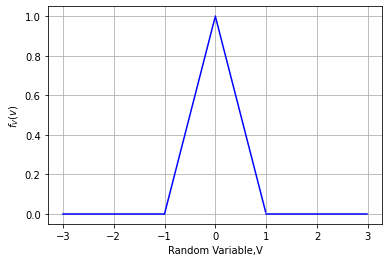
\includegraphics[width=\columnwidth] {Assignment_3_Fig_1.png}
    \caption{The PDF of V}
    \label{fig:The PDF of V}
\end{figure}

The CDF of V is defined as,
\begin{equation}
    F_V(v) = \Pr\brak{V \le v}
\end{equation}
Now for $ v \le 0 $,
 \begin{align}
    \Pr\brak{V\le v} &=  \int_{-\infty}^{v}f_{V}(v) \,dv  \\
          &=  \int_{-1}^{v} (1+v) \,dv  \\
          &=  \left(\dfrac{v^2}{2}+v \right) \Biggr|_{-1}^{v}  \\
          &=   \left(\left(\dfrac{v^2}{2}+v \right) - \left(\dfrac{1}{2} -1 \right)\right) \\
          &= \dfrac{v^2+2v +1}{2}
\end{align}
Similarly for $v \le 1$,
\begin{align}
    \Pr\brak{V\le v} &=  \int_{-\infty}^{v}f_{V}(v) \,dv  \\
          &=  \dfrac{1}{2} + \int_{0}^{v}(1-v)\,dz  \\
          &=  \dfrac{-v^2+2v+1}{2}
\end{align}

The CDF is as below: 
\begin{align}
\label{eq:cdf_v}
F_{V}(v)  = 
\begin{cases}
0 & v < -1
\\
\dfrac{v^2+2v + 1}{2} &  v \le 0
\\
\dfrac{-v^2+2v+1}{2} &  v \le 1
\\
1 & v > 1
\end{cases}
\end{align}

The plot for CDF of $V $ can be observed at figure \ref{fig:The CDF of V}\\

\begin{figure}[!ht]
       \centering
    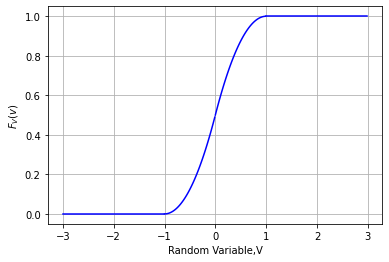
\includegraphics[width=\columnwidth] {Assignment_3_Fig_2.png}
    \caption{The CDF of V}
    \label{fig:The CDF of V}
\end{figure}

We need  $\pr{Z-W >\frac{1}{2}}$ where $Z = max(X,Y)$ and $W = min(X,Y)$. Now,

\begin{align}
\label{eq:pdf_v}
Z-W  = 
\begin{cases}
X-Y & \text{for } X \geq Y
\\
Y-X & \text{for } X < Y
\end{cases}
\end{align}

Therefore,
\begin{align}
    \pr{Z-W >\frac{1}{2}} &= \pr{X-Y>\frac{1}{2},X \geq Y} \nonumber \\
    &+\pr{Y-X > \frac{1}{2}, X < Y}\\
    &= \pr{X-Y>\frac{1}{2}} +\pr{Y-X>\frac{1}{2}}\\
    &= \pr{V > \frac{1}{2}} + \pr{-V > \frac{1}{2}}\\
    &= 1 - \pr{V \leq \frac{1}{2}} + \pr{V < \frac{-1}{2}}\\
    &= 1-F_V(\frac{1}{2}) + F_V(-\frac{1}{2})\\
    &= 1 -\frac{7}{8} + \frac{1}{8}\\
    &= \frac{1}{4}
\end{align}

Hence the correct answer is option (C).
\end{document}
